\section{Expected perfomance on other platforms}
\label{sec-evaluation-other-platforms}
Platform independence is one of the main advantages of using a VM. The AVR family of CPUs is widely used in low power embedded systems, and we implemented our VM for the ATmega128 CPU. However, our approach does not depend on any AVR specific properties and the approach described in this dissertation can be applied on other embedded CPU platforms to improve performance and provide a safe execution environment. The main requirements are the ability to reprogramme its own programme memory, and the availability of a sufficient number of registers for stack caching.

While it is impossible to determine exactly what the resulting performance would be on different platforms without porting the VM, we present some results here that indicate it is likely to be worse than the results we see on the ATmega.

Two parameter that are of important influence to our VM are the number of available registers and the size of the registers. Table \ref{tbl-ATmega-msp430-m0-registers} lists these parameter for the ATmega, and two other common families of embedded CPUs, the Texas Instruments MSP430 and ARM Cortex-M0. These CPUs are similar in many ways, including the amount of RAM and flash memory typically available, but differ in the number of registers and word size.

\begin{table}
\caption{Number or registers and word size for the ATmega, MSP430, and Cortex M0}
\label{tbl-ATmega-msp430-m0-registers}
    \begin{tabular}{lrrr} % NO SIMULATION DATA
    \toprule
                                           & ATmega       & MSP430     & Cortex M0 \\
                                           & \cite{Atmel:ATmega128Datasheet, Atmel:AVRInstructionSetManual}
                                           & \cite{TexasInstrumentsIncorporated:MSP430F1611Datasheet, TexasInstrumentsIncorporated:MSP430x1xxUsersGuide}
                                           & \cite{ARM:2009vz} \\
    \midrule
    \midrule
    Number of general purpose registers    & 32           & 12         & 13        \\
    Word size                              & 8-bit        & 16-bit     & 32-bit    \\
    Total register file size (bytes)       & 32           & 24         & 52        \\
    \bottomrule
    \end{tabular}
\end{table}

\subsection{Number of registers}

\begin{figure}
\centering
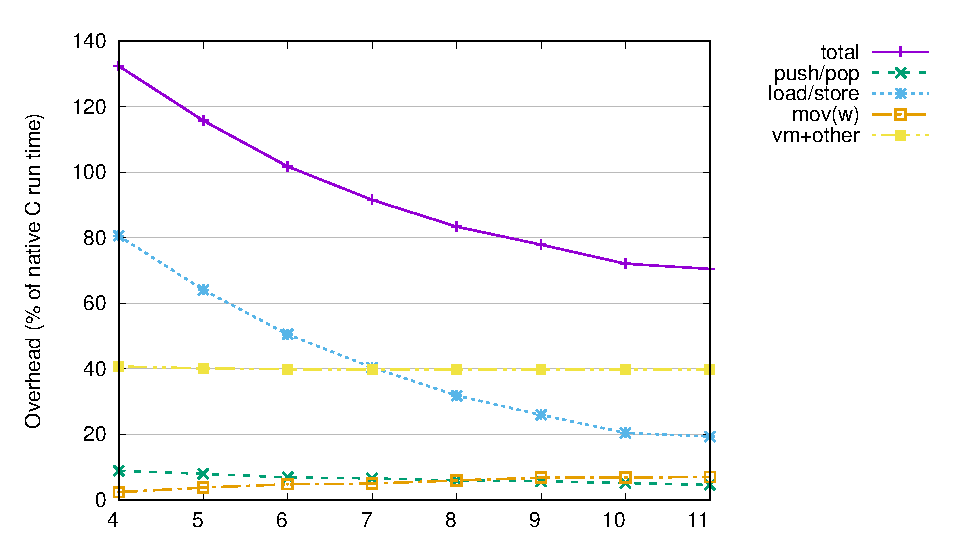
\includegraphics[width=\mygraphsize]{cachesize-performance-per-opcode-category.eps}
\caption{Performance for different stack cache sizes (in pairs of registers)}
\label{fig-performance-per-opcode-category-per-cachesize}
\end{figure}

\begin{table}
\caption{Performance overhead for different stack cache sizes (in pairs of registers)}
\label{tbl-performance-per-opcode-category-per-cachesize}
    \begin{tabular}{lrrrrrr} % UPDATED 20180327
    \toprule
    Number of                      & \multicolumn{5}{l}{Overhead} \\
    register pairs                 &  push/pop &   load/store &      mov(w) &    vm+other & \makebox[0.2mm]{}   &   total \\
    \midrule
    \midrule
      4                            &       8.7 &         80.5 &         2.4 &        38.1 &                     &   129.7 \\
      5                            &       7.8 &         64.0 &         3.8 &        37.5 &                     &   113.0 \\
      6                            &       6.7 &         50.3 &         4.7 &        37.0 &                     &    98.7 \\
      7                            &       6.4 &         40.2 &         4.9 &        37.0 &                     &    88.4 \\
      8                            &       5.7 &         31.6 &         5.8 &        36.9 &                     &    80.1 \\
      9                            &       5.5 &         25.6 &         6.7 &        36.9 &                     &    74.6 \\
     10                            &       4.9 &         20.1 &         6.8 &        36.9 &                     &    68.7 \\
     11                            &       4.3 &         18.9 &         6.9 &        36.9 &                     &    67.0 \\
    \bottomrule
    \end{tabular}
\end{table}


The ATmega has 32 8-bit registers available, which we manage as 16 pairs since our VM stores data in 16-bit slots. Looking at the MSP430, it only has 12 registers, but they are 16-bit. 5 register pairs are reserved on the ATmega, leaving us with 11 pairs available for stack caching. If we can achieve the same by reserving 5 16-bit registers on the MSP430, 7 registers will be available to the stack cache.

To evaluate the effect of a smaller number of registers on the stack cache, all benchmarks were run while restricting the number of registers the cache manage may use. Since our approach needs a minimum of 4 pairs, we vary the number of register from 4 to 11.

The results are shown in Figure \ref{fig-performance-per-opcode-category-per-cachesize} and Table \ref{tbl-performance-per-opcode-category-per-cachesize}. As is common with caching techniques, the first few registers have the most impact, with half of the overhead reduction already realised when adding the first two additional registers. Ignoring all other difference for the moment, the effect of reducing the number of register pairs from 11 to 7 is an increase in overhead by 20.8\%, to 92.0\%.

The Cortex M0 has one general purpose register more than the MSP430, and at 8 register pairs the overhead drops to 84.1\%. In addition, the M0's registers are 32-bit, which means in cases where mostly 32-bit values are used, the stack size is effectively doubled since values can be stored in a single register instead of two pairs of 8-bit registers.

A final interesting thing to note in Figure \ref{fig-performance-per-opcode-category-per-cachesize} is the fact the increasing the cache size mostly reduces the load/store overhead. Using only 4 pairs, stack caching has already removed most of the push/pop overhead, which only drops slightly when more registers are used. However, these extra registers reduce load/store overhead significantly since more registers are available for the markloop optimisation, and using more registers it increases the chance that an old, popped value may still be present, allowing popped value caching to eliminate more loads.

\subsection{Word size}
\label{sec-evaluation-other-platforms-word-size}

\begin{figure}
\centering
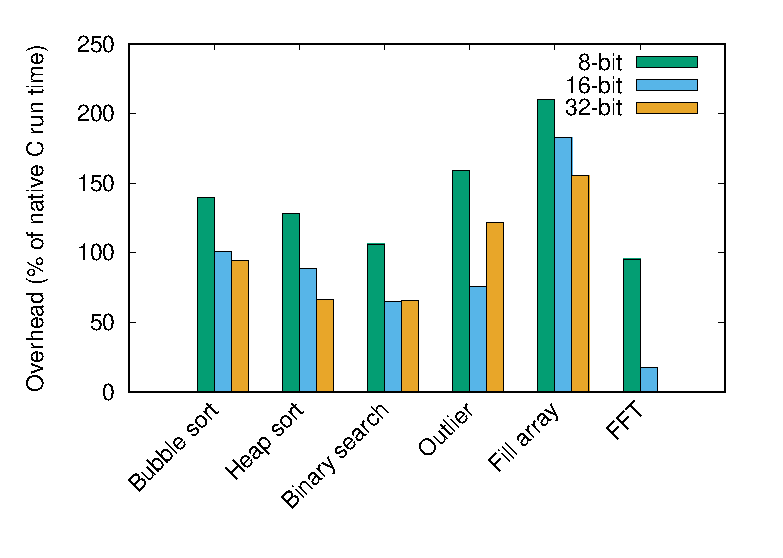
\includegraphics[width=\mygraphsize]{8_16_32_bit.eps}
\caption{Performance for different data sizes}
\label{fig-performance-8-16-32-bit}
\end{figure}

% UPDATED 20180214

\begin{table}[]
\centering
\caption{Performance for different data sizes}
\label{tbl-performance-8-16-32-bit}
\begin{tabular}{lrrr}
\toprule
               &   8-bit  &  16-bit  &     32-bit \\
\midrule
Bubble sort    &    139.5 &    101.2 &       94.4 \\
Heap sort      &    128.4 &     88.5 &       66.2 \\
Binary search  &    106.3 &     65.2 &         66 \\
Outlier        &      159 &     75.7 &      121.6 \\
FFT            &     96.7 &     17.7 &            \\
\bottomrule
\end{tabular}
\end{table}


A second important difference between the CPUs in Table \ref{tbl-ATmega-msp430-m0-registers} is the size of the registers. The main measure to evaluate our approach has been the overhead compared to native C performance or code size. While having a large register size is good for absolute performance, we expect it to hurt the \emph{relative} performance of our VM.

A number of benchmarks can be implemented using different data sizes. As mentioned in Section \ref{sec-evaluation-benchmarks}, 16-bit data is used in the main evaluation. Figure \ref{fig-performance-8-16-32-bit} and Table \ref{tbl-performance-8-16-32-bit} show the resulting performance for 8, 16, and 32-bit versions of these benchmarks (no 32-bit version of the \mycode{fix\_fft.c} code was available).

In almost all cases, a smaller data size results in a slower performance. This is because using larger data sizes increases the time spent in code that is common to both C and AOT versions. Taking \mybench{bubble sort} as an example, both versions do the same number of array loads, comparisons, and array stores. When operating on 32-bit data, this takes twice as long as for 16-bit data. In addition the AOT version introduces overhead, in \mybench{bubble sort}'s case primarily from calculating array element locations (see Section \ref{sec-evaluation-bubble-sort}). For a 32-bit array, this takes 17 cycles, 8 of which are spent on the actual load or store, but for 16-bit array access this is only 4 out of 13 cycles.

This effect is even clearer for more complex operations like multiplication. 16x16 to 16-bit multiplication can be implemented in a few instructions and only takes 10 cycles on the ATmega. 32x32 to 32-bit multiplication is implemented by calling \mycode{avr-gcc}'s \mycode{\_\_mulsi3} function, and takes 85 to 100 cycles.

Thus, working with 16-bit or 32-bit data on an 8-bit CPU helps the compiler's relative performance by introducing a larger common component that both C and AOT compiled versions have to execute. On the MSP430 or Cortex M0, that operate on 16-bit or 32-bit values in a single step, this effect will be reduced or eliminated. The exact impact of this is hard to estimate, but it is likely to be in the order of tens of percents extra overhead.

In Table \ref{tbl-performance-8-16-32-bit} we see the \mybench{outlier detection} benchmark performs worse for 32-bit data compared to 16-bit data. This is due to a mismatch between the infuser and ProGuard. In JVM byte code, local variables are stored in 32-bit slots. The code generated by \mycode{javac} uses a separate slot for each variable, but ProGuard attempts to reduce memory consumption by mapping multiple variables to the same slot if their live ranges do not overlap. The infuser processes the ProGuard optimised code, as shown in Figure \ref{fig-translation-process}, and replaces the JVM's 32-bit operations by 16-bit versions where possible. In the 32-bit \mybench{outlier detection} benchmark, ProGuard mapped a 32-bit and 16-bit variable to the same slot, which prevents the infuser from using the cheaper 16-bit operations for this variable. This once again highlights the need for a unified, optimising compiler, combining the tasks of \mycode{javac}, ProGuard and the Darjeeling infuser.

The large difference in performance for \mybench{FFT} is mostly due to bit shifts. The 8-bit version does many shifts of a 16-bit value by exactly 6 bits. Our VM simply emits 6 single-bit shifts, while \mycode{avr-gcc} has a special optimised version for this case, which we considered too specific to include in our VM. The 32-bit version spends about half of its time shifting a 32-bit value by 15 bits, The VM and \mycode{avr-gcc} both implement this using the same loop, which again adds a large common factor, thus reducing the relative overhead.


%JVM_GETARRAY_I                                                  554880  18.2%  35.3%C      32640  17.0 |    1    24   7.8%  15.8%C 4->4:Int 
%1        movw r30, r6    -> 0x010E2E: movw r30, r6                32640                     32640
%1        add r30, r30    -> 0x010E30: add r30, r30                32640                     32640
%1        adc r31, r31    -> 0x010E32: adc r31, r31                32640                     32640
%1        add r30, r30    -> 0x010E34: add r30, r30                32640                     32640
%1        adc r31, r31    -> 0x010E36: adc r31, r31                32640                     32640
%1        add r30, r4     -> 0x010E38: add r30, r4                 32640                     32640
%1        adc r31, r5     -> 0x010E3A: adc r31, r5                 32640                     32640
%2        adiw r30, 3     -> 0x010E3C: adiw r30, 3                 65280                     32640
%
%2        ldpi r22, Z     -> 0x010E3E: ldpi r22, Z                 65280                     32640
%2        ldpi r23, Z     -> 0x010E40: ldpi r23, Z                 65280                     32640
%2        ldpi r20, Z     -> 0x010E42: ldpi r20, Z                 65280                     32640
%2        ld r21, Z       -> 0x010E44: ld r21, Z                   65280                     32640
%overhead: 9, load 8
%
%JVM_GETARRAY_S                                                  359040  18.2%  36.6%C      32640  11.0 |    1    16   6.2%  13.6%C 4->2:Short 
%1        movw r30, r6    -> 0x010DF2: movw r30, r6                32640                     32640
%1        add r30, r30    -> 0x010DF4: add r30, r30                32640                     32640
%1        adc r31, r31    -> 0x010DF6: adc r31, r31                32640                     32640
%1        add r30, r4     -> 0x010DF8: add r30, r4                 32640                     32640
%1        adc r31, r5     -> 0x010DFA: adc r31, r5                 32640                     32640
%2        adiw r30, 3     -> 0x010DFC: adiw r30, 3                 65280                     32640
%
%2        ldpi r24, Z     -> 0x010DFE: ldpi r24, Z                 65280                     32640
%2        ld r25, Z       -> 0x010E00: ld r25, Z                   65280                     32640
%
%overhead: 7, load 4

